\subsection{ASL-Skeleton3D}
\label{sec:metodologia-datasets-3d}

O ASL-Skeleton3D é um \dataset intermediário oriundo deste trabalho que introduz a representação em coordenadas 3D das amostras do \acrshort{asllvd}. Esse tipo de representação possibilita uma observação mais precisa do corpo dos indivíduos enquanto articulam os sinais, permitindo a pesquisadores em \acrshort{slr} explorar novas técnicas ou derivar outros \datasets computados a partir dessas coordenadas.

A estratégia adotada para projetar os sinais do \acrshort{asllvd} dentro do espaço 3D consistiu em combinar duas de suas perspectivas 2D capturadas por câmeras posicionadas perpendicularmente entre si: a vista frontal e a vista lateral. Com isso, a vista frontal fornecerá a observação dos eixos \(x\) e \(y\), e a vista lateral nos fornecerá a dimensão de profundidade (ou eixo \( z\)), conforme ilustra a \autoref{fig:our-strategy-3d}.

\begin{figure}[ht!]
    \centering
    \caption{\textmd{Estratégia adotada para representar os sinais no espaço 3D: as visões 2D para a frente~(\subref{subfig:our-strategy-3d-front}) e lateral~(\subref{subfig:our-strategy-3d-side}) são posicionadas perpendicularmente para reconstruir a visão 3D do objeto~(\subref{subfig:our-strategy-3d-persp}).}}
    \subcaptionbox{\label{subfig:our-strategy-3d-front}}{
        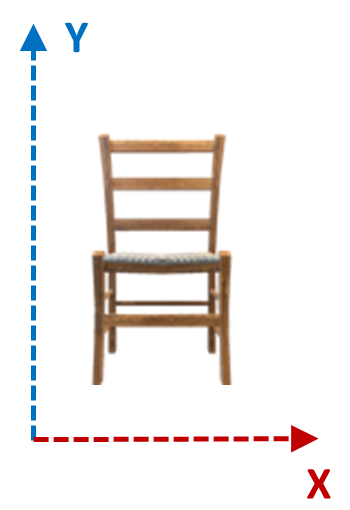
\includegraphics[height=4cm]{imagens/metodologia/datasets/chair_front}
    }%
    \hfill
    \subcaptionbox{\label{subfig:our-strategy-3d-side}}{
        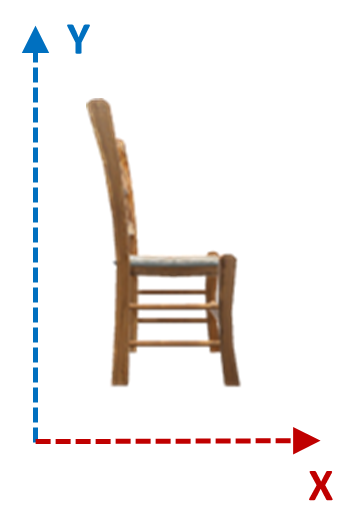
\includegraphics[height=4cm]{imagens/metodologia/datasets/chair_side}
    }%
    \hfill
    \subcaptionbox{\label{subfig:our-strategy-3d-persp}}{
        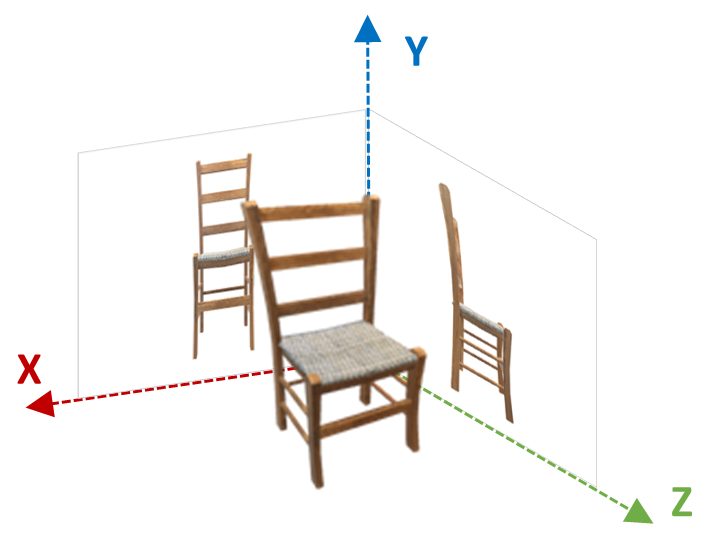
\includegraphics[height=4cm]{imagens/metodologia/datasets/chair_perspective}
    }%
    \nomefonte{}
    \label{fig:our-strategy-3d}
\end{figure}


Os passos utilizados para gerar o ASL-Skeleton3D basearam-se no processamento realizado por \citeonline{amorim-2019-stgcn-sl} na construção de um \dataset de esqueletos 2D da \acrshort{asl}. De um modo geral, eles envolvem a obtenção das amostras, a segmentação dos sinais, a estimativa e a normalização dos esqueletos. Apesar disso, várias adaptações foram necessárias a cada passo para acomodar a estratégia descrita acima e lidar com os desafios encontrados aqui, conforme discutiremos a seguir:

\begin{enumerate}
    \item \textbf{Obtenção das amostras}: essa etapa consiste em recuperar as amostras de vídeos do \acrshort{asllvd}, porém considerando duas câmeras -- frontal e lateral -- para aplicar a estratégia descrita acima. Existem dois formatos originalmente disponíveis para as câmeras: \textit{mov} (vídeos compactados, geralmente menores e mais fáceis de processar) e \textit{vid} (vídeos brutos, mais longos para baixar e processar).

          Ao analisar as amostras, identificamos que parte delas possuía as duas câmeras disponíveis em ambos os formatos; para outras, havia ambas câmeras, mas cada uma estava em um formato distinto; nos piores casos, contudo, faltava uma das câmeras ou ela estava corrompida, fazendo com que essas amostras precisassem ser descartadas. Lidar com isso acrescentou uma complexidade extra, mas que foi contornada com uma perda de apenas 0,16\% das amostras originais -- resultando num total de 9.747 amostras.

          % -----
    \item \textbf{Segmentação dos sinais}: consiste em segmentar as sequências de vídeos do \acrshort{asllvd}, que são extensas e contemplam múltiplos sinais, em pedaços menores com apenas um sinal. Nesse processo, reduzimos a taxa de quadros de 60 para 3 FPS uma vez que, dadas as condições em que os indivíduos foram filmados, assumimos que eles não conseguiriam realizar mais de três movimentos em um único segundo -- consequentemente, muitos dos frames originais conteriam informação duplicada. Isso também nos ajudou a reduzir em cerca de 20 vezes o número de frames a serem processados nas etapas posteriores.

          % -----
    \item \textbf{Estimativa dos esqueletos 3D}: aqui realizamos a estimativa dos esqueletos dos sinalizadores utilizando o OpenPose~\cite{cao-2019-openpose,simon-2017-openpose-hand-face}. Isso foi feito para ambas as câmeras frontal e lateral, o que nos rendeu dois esqueletos 2D:

          \begin{enumerate}
              \item \textit{Esqueleto frontal}, contendo as coordenadas plotadas sobre o eixos \(x\) e \(y\) (vide \autoref{subfig:front-side-persp-skeletons-front}).
                    Essas coordenadas descrevem a mesma visão frontal que esperamos obter ao imaginar o nosso esqueleto 3D final observado de frente. Por conta disso, utilizamos essas coordenadas \(x\) e \(y\) da forma como são fornecidas para ancorar o indivíduo no espaço tridimensional. Precisaremos apenas adicionar a dimensão de profundidade.

              \item \textit{Esqueleto lateral}, que também contém um par de coordenadas \(x\) e \(y\) (vide \autoref{subfig:front-side-persp-skeletons-side}).
                    No entanto, vamos aplicar a estratégia descrita acima e posicioná-lo perpendicularmente ao esqueleto frontal (como no ~\autoref{subfig:front-side-persp-skeletons-persp}). Nesse caso, observamos que embora o eixo \(y\) fornecido aqui contenha as mesmas coordenadas que no esqueleto frontal, o eixo \(x\) descreverá coordenadas equivalentes às de profundidade. Dessa forma, tomaremos o eixo \(x\) do esqueleto lateral como sendo o eixo \(z\) (eixo de profundidade) para o nosso esqueleto 3D final.
          \end{enumerate}

          \begin{figure}[ht!]
              \centering
              \caption{\textmd{As coordenadas \(x\) e \(y\) do esqueleto 3D final são obtidas das coordenadas estimadas para a perspectiva frontal~(\subref{subfig:front-side-persp-skeletons-front}). A coordenada \(z\) é originada do eixo \(x\) do esqueleto lateral~(\subref{subfig:front-side-persp-skeletons-side}). Quando colocados juntos, eles são visualizados como em (\subref{subfig:front-side-persp-skeletons-persp}).}}
              \subcaptionbox{\label{subfig:front-side-persp-skeletons-front}}{
                  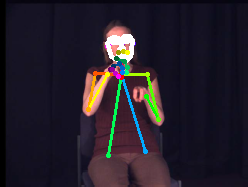
\includegraphics[height=3cm]{imagens/metodologia/datasets/asllvd_example_front_skeleton}
              }%
              \hfill
              \subcaptionbox{\label{subfig:front-side-persp-skeletons-side}}{
                  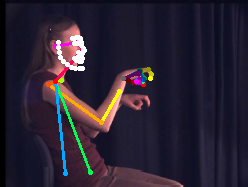
\includegraphics[height=3cm]{imagens/metodologia/datasets/asllvd_example_side_skeleton}
              }%
              \hfill
              \subcaptionbox{\label{subfig:front-side-persp-skeletons-persp}}{
                  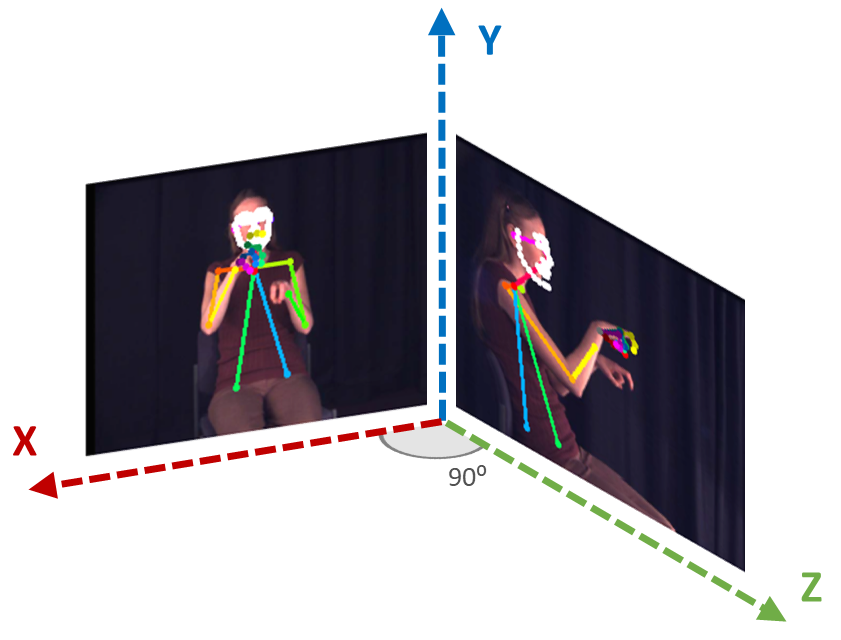
\includegraphics[height=4.5cm]{imagens/metodologia/datasets/asllvd_front_side_perspective_skeleton}
              }%
              \nomefonte{}
              \label{fig:front-side-persp-skeletons}
          \end{figure}

          % -----
    \item \textbf{Normalização dos esqueletos 3D}: no último passo, normalizamos os esqueletos 3D para remover variações decorrentes do posicionamento das câmeras e diferenças nos corpos dos indivíduos. Isso é importante porque o \acrshort{asllvd} foi capturado em diferentes seções e envolvendo diferentes sinalizadores.

          \figura
          {fig:shoulders-width} % Label
          {imagens/metodologia/datasets/shoulders_width} % Path
          {height=3cm} % Size
          {Largura entre ombros, que foi utilizada como referência para normalizar as coordenadas nos esqueletos 3D.} % Caption
          {} % Citation

          Para isso, adotamos como referência a largura entre os ombros dos sinalizadores (vide \autoref{fig:shoulders-width}), a qual foi inspirada pela medida antropométrica \textit{diâmetro biacromial} \cite{stoudt-1970-skinfolds}. Dessa forma, a largura dos ombros \(W_{shoulders}\) é calculada através da distância euclidiana \(d\) \cite{anton-2013-algebra} entre as coordenadas do ombro esquerdo \(S_{l}\) e direito \(S_ {r}\), como na \autoref{eqn:shoulders-width}:

          \begin{equation}
              \label{eqn:shoulders-width}
              W_{shoulders} = d\left(S_{l}, S_{r}\right)
          \end{equation}

          Uma vez que \(W_{shoulders}\) foi calculado, podemos então transformar cada coordenada \(K\) em sua respectiva versão normalizada \(K_{norm}\), conforme \autoref{eqn:normalized-keypoint}:

          % Normalização de pontos-chave:
          \begin{equation}
              \label{eqn:normalized-keypoint}
              K_{norm} = \frac{K}{W_{shoulders}}
          \end{equation}

\end{enumerate}


A \autoref{fig:sample-json-datasetTD} exemplifica uma amostra do ASL-Skeleton3D, bem como as propriedades fornecidas para ela. Observam-se no início do arquivo algumas propriedades com informações básicas extraídas do \acrshort{asllvd}, como rótulo, consultor, sessão, cena, frames de início e fim, entre outras. Além disso, temos a propriedade ``frames'', que contém a lista de frames da amostras e os esqueletos estimados para cada um deles. Cada frame contém grupos que correspondem às partes do corpo e, dentro desses grupos, estão as coordenadas contendo seu respectivo nome, um \textit{score} que identifica a acurácia da estimativa daquela coordenada, e os eixos \(x\), \(y\) e \(z\).
Por exemplo, se observarmos o segundo índice de cada um dos arrays contidos no grupo \textit{body} (do corpo do sinalizador), notaremos que ele corresponde à coordenada \textit{neck} (do pescoço), a qual possui um \textit{score} de 62\% e coordenadas \(x\), \(y\) e \(z\) localizadas em 4,469, 2,871 e 1,898, aproximadamente.

\figura
    {fig:sample-json-datasetTD} % Label
    {imagens/metodologia/datasets/code_3d} % Path
    {width=0.7\linewidth} % Size
    {Exemplo de amostra do ASL-Skeleton3D e propriedades fornecidas para ela.} % Caption
    {} % Citation

Por fim, o \textit{dataset} resultante do processamento acima, bem como o código-fonte utilizado para isso, está disponível publicamente na URL listada abaixo\footnote{Disponível em \url{http://www.cin.ufpe.br/~cca5/asl-skeleton3d}}.
